\documentclass[a4paper,10pt]{article}

\usepackage{graphicx}
\usepackage[T2A]{fontenc}
\usepackage[utf8]{inputenc}
\usepackage[english,russian]{babel}
\usepackage{amssymb}
\usepackage{wrapfig}

\RequirePackage{caption}
\DeclareCaptionLabelSeparator{defffis}{ — }
\captionsetup{justification=centering,labelsep=defffis}

\usepackage{caption} \captionsetup[table]{labelsep=endash,justification=justified,singlelinecheck=false,font=normalsize}

\usepackage{amsmath,amsfonts,amssymb,amsthm,mathtools}



\begin{document}
  
\begin{center}
  \section*{Лабораторная работа №3.1.3 \\Измерение магнитного поля Земли\\Джокер Бэтмен, Б02-000, 18.09.2021}
\end{center}  

\vspace{5mm}
\section*{Введение}

\begin{flushleft}
  \textbf{Цель работы:} исследовать свойства постоянных неодиомвых магнитов, измерить с их помощью горизонтальную и вертикальную составляющие инукции магнитного поля Земли и магнитное наклонение.

\end{flushleft}

\begin{flushleft}
  \textbf{В работе используются:} неодимовые магниты; тонкая нить для изготовления крутильного маятника; медная проволока; электронные весы; секундомер; измеритель магнитной индукции; штангенциркуль; брусок, линейка и штатив из немагнитных материалов; набор гирь и разновесов.

\end{flushleft}

\section*{Теоретическая справка}

Простейший магнитный диполь может быть образован витком с током или постоянным магнитом. По определению, магнитный момент $\vec{\mathfrak{m}}$ тонкого витка площадью $S$ с током $I$ равен (в СИ)\[\vec{\mathfrak{m}}=I\vec{S},\]где $\vec{S}=S\vec{n}$ -- вектор площади контура, образующий с направлением тока правовинтовую систему, $\vec{n}$ -- единичный вектор нормали к площадке (это же направление $\vec{\mathfrak{m}}$ принимается за направление $S\to N$ от южного $S$ к северному $N$ полюсу магнита). Если размеры контура с током или магнитной стрелки малы по сравнению с расстоянием до диполя, то соответствующий магнитный диполь $\vec{\mathfrak{m}}$ называют \textit{элементраным} или \textit{точечным}.

Магнитное поле точечного диполя определяется по формуле, аналогичной формуле для поля элементарного электрического диполя:\[\vec{B}_{\text{дип}}=\frac{\mu_0}{4\pi}\left(\frac{3\left(\vec{\mathfrak{m}}\cdot\vec{r}\right)\vec{r}}{r^5}-\frac{\vec{\mathfrak{m}}}{r^3}\right).\]

Во внешнем магнитном поле с индукцией $\vec{B}$ на точечный магнитный диполь $\vec{\mathfrak{m}}$ действует механический момент сил\[\vec{\mathcal{M}}=\left[\vec{\mathfrak{m}}\times\vec{B}\right].\]При этом потенциальная энергия, которой обладает диполь с постоянным $\vec{\mathfrak{m}}$, равна\[W=-\left(\vec{\mathfrak{m}}\cdot\vec{B}\right).\]Когда диполь ориентирован вдоль внешнего поля ($\mathfrak{m}\parallel\vec{B}$), он находится в состоянии \textit{равновесия} ($\vec{\mathcal{M}}=0$). При этом \textit{устойчивым} будет только состояние, в котором диполь \textit{сонаправлен} с полем $\vec{\mathfrak{m}}\uparrow\uparrow\vec{B}$, поскольку его потенциальная энергия достигает \textit{минимума} $(W_{min}=-\mathfrak{m}B)$. При противоположной ориентации энергия будет иметь максимум $W_{max}=\mathfrak{m}B$, и состояние равновесия будет неустойчивым.

В \textit{неоднородном} внешнем поле выражение для энергии постоянного диполя сохраняется. При этом кроме момента сил на диполь действует ещё и сила\[\vec{F}=-\nabla W=\left(\vec{\mathfrak{m}}\cdot\nabla\right)\vec{B}.\]В частности, проекция этой силы на ось $x$ имеет вид\[F_x=\mathfrak{m}_x\frac{\partial B_x}{\partial x}+\mathfrak{m}_y\frac{\partial B_y}{\partial y}+\mathfrak{m}_z\frac{\partial B_z}{\partial z}.\]Таким образом, \textit{свободный} магнитный диполь в неоднородом магнитном поле ориентируется вдоль силовых линий магнитного поля и втягивается в область более сильного поля, поскольку это ведёт к уменьшению энергии диполя.

Рассчитаем силу взаимодействия магнитов с моментами $\vec{\mathfrak{m}}_1$ и $\vec{\mathfrak{m}}_2$ в рамках модели точечных диполей. В частном случае, когда моменты двух небольших магнитов направлены вдоль соединяющей их прямой: $\vec{\mathfrak{m}}_{1,2}\parallel\vec{r}$, где $\vec{r}$ -- радиус-вектор между ними, магниты взаимодействуют с силой\[F_{12}=\mathfrak{m}_1\frac{\partial B_2}{\partial r}=\mathfrak{m}_1\frac{\partial\left(\frac{2\mathfrak{m}_2}{r^3}\right)}{\partial r}=-\frac{6\mathfrak{m}_1\mathfrak{m}_2}{r^4}\ \text{(ед. СГС).}\]Здесь магниты притягиваются, если их магнитные моменты сонаправлены $(\vec{\mathfrak{m}}_1\uparrow\uparrow\vec{\mathfrak{m}}_2)$, и отталкиваются, если направлены противоположно $(\vec{\mathfrak{m}}_1\uparrow\downarrow\vec{\mathfrak{m}}_2)$.

Если магнитные моменты направлены перпендикулярно соединяющей их прямой: $\vec{\mathfrak{m}}_{1,2}\perp\vec{r}$, то нетрудно показать, что сила их взаимодействия окажется в два раза меньшей и будет иметь противоположный знак:\[F_{12}=\frac{3\mathfrak{m}_1\mathfrak{m}_2}{r^4}\ \text{(ед. СГС)}\](диполи притягиваются при $\vec{\mathfrak{m}}_1\uparrow\downarrow\vec{\mathfrak{m}}_2$ и отталкиваются при $\vec{\mathfrak{m}}_1\uparrow\uparrow\vec{\mathfrak{m}}_2$).

Для проведения эксперимента важно, что, во-первых, вещество, из которого изготовлены магниты, является \textit{магнитожёстким} материалом, и, во-вторых, шары намагничены однородно.

"Магнитожёсткость" материала означает, что магнитные моменты шаров в процессе работы не изменяются под действием внешних магнитных полей, т. е. шар ведёт себя как постоянный ("жёсткий") диполь. В том числе, магнитные моменты не изменяются при контакте магнитов друг с другом.

Магнитное поле однородно намагниченного шара радиусом $R$ может быть вычислено точно. На расстояниях $r\geq R$ от центра шара оно совпадает с полем точечного магнитного диполя, расположенного в центре, магнитный момент $\mathfrak{m}$ которого совпадает с полным моментом шара. Внутри шара магнитное поле однородно -- нетрудно получить, что при $r < R$\[\vec{B}_0=\frac{\mu_0\vec{\mathfrak{m}}}{2\pi R^3}\ \left[\text{СИ}\right].\]

В качестве ещё одной характеристики материала магнита используют остаточную \textit{намагниченность} $\vec{M}$. По определению, намагниченность равна \textit{объёмной плотности магнитного момента}, поэтому для однородно намагниченного шара\[\vec{\mathfrak{m}}=\vec{M}V,\]где $V=\frac{4\pi}{3}R^3$ -- объём магнита. Величину $\vec{B}_r=\mu_0\vec{M}$ называют \textit{остаточной индукцией} материала.

Нетрудно видеть, что индукция $\vec{B}_p$ \textit{на полюсах} однородно намагниченного шара неправлена по нормали к поверхности и совпадает поэтому с индукцией внутри шара: $\vec{B}_p=\vec{B}_0$. Тогда величина $B_p$ связана с остаточной индукцией $B_r$ соотношением\[B_p=B_0=\frac{2}{3}B_r.\]

\section*{Экспериментальная установка}

\subsection*{Определение величины магнитного момента шариков}

Величину магнитного момента $\mathfrak{m}$ одинаковых шариков можно рассчитать, зная их массу $m$ и определив максимальное расстояние $r_{max}$, на котором они ещё удерживают друг друга в поле тяжести. При максимальном расстоянии сила тяжести шариков равна силе их магнитного притяжения:\[\frac{6\mathfrak{m}^2}{r_{max}^4}=mg\implies\mathfrak{m}=\sqrt{\frac{mgr_{max}^4}{6}}.\]

По величине магнитного момента $\mathfrak{m}$ можно рассчитать величину индукции магнитного поля вблизи любой точки на поверхности шара радиуса $R$. Максимальная величина индукции наблюдается на полюсах:\[\vec{B}_p=\frac{2\vec{\mathfrak{m}}}{R^3}.\]

Величину магнитного момента шариков можно определить макже по силе их сцепления. Она определяется как сила, необходимая для разрыва двух сцепившихся магнитных шариков. Сила сцепления максимальна, если шары соединяются своими противоположными полюсами.

Максимальную силу сцепления можно определить по весу магнитной цепочки, которую способен удержать самый верхний магнитный шарик. Если цепь состоит из одинаковых магнитных шариков, то при определённой длине она она оторвётся от верхнего шарика. Приэтом, учитывая, что сила приятжения убывает как $F\sim\frac{1}{r^4}$, для расчёта прочности цепочки достаточно учитывать силу взаимодействия верхенего шара с тремя-четырьмя ближайшими соседями.

Если сила сцепления двух одинаковых шаров диаметром $d$ с магнитными моментами $\mathfrak{m}$ равна\[F_0=\frac{6\mathfrak{m}^2}{d^4},\]то минимальный вес цепочки, при которой она оторвётся от верхнего шарика, равен\[F=F_0\sum_{n=1}^{+\infty}\frac{1}{n^4}=\frac{\pi^4}{90}F_0\approx1,08F_0.\]

Таким образом, сила сцепления двух шаров равна\[F_0=\frac{90}{\pi^4}F=0,924F.\]

\subsection*{Измерение горизонтальной составляющей индукции магнитного поля Земли}

Магнитное поле в настоящей работе определяется по периоду крутильных колебаний магнитной стрелки вокруг вертикальной оси.

"Магнитная стрелка" образована из сцепленных друг с другом противоложными полюсами шариков и с помощью $\Lambda$-образного подвеса подвешена в горизонтальном положении. Магнитные моменты шариков направлены в одну сторону вдоль оси "стрелки". Под действием вращательного момента $\vec{M}=\vec{\mathfrak{m}}_0\times\vec{B}$ магнитный момент "стрелки" $\vec{\mathfrak{m}}_0$ выстроится вдоль горизонтальной составляющей магнитного поля Земли $\vec{B}_h$ в направлении $S\to N$. При отклонении "стрелки" на угол $\theta$ от равновесного положения в горизонтальной плоскости возникают крутильные колебания вокруг вертикальной оси, проходящей через середину "стрелки". Если пренебречь упругостью нити, то уравнение крутильных колебаний такого маятника при малых амплитудах ($\sin{\theta}\approx\theta$) имеет вид\[I_n\ddot{\theta}+\mathfrak{m}_0B_h\theta=0,\]где $I_n=\frac{1}{12}m_{\text{ст}}l_{\text{ст}}^2=\frac{1}{12}n^3md^2$ -- момент инерции "стрелки" , состоящей из $n$ шариков, который можно с хорошей точностью приблизить моментом инерции тонкого однородного стержня соответствующей массы и длины, а $\mathfrak{m}_0=n\mathfrak{m}$ -- полный магнитный момент стрелки.

Таким образом, период колебаний маятника оказывается равен\[T(n)=2\pi\sqrt{\frac{md^2}{3\mathfrak{m}B_h}}n=kn,\]где $k=2\pi\sqrt{\frac{md^2}{3\mathfrak{m}B_h}}$.

\subsection*{Измерение вертикальной составляющей индукции магнитного поля Земли. Магнитное наклонение.}

Для измерения вертикальной составляющей $B_v$ вектора индукции поля Земли используется та же установка, что и для измерения горизонтальной составляющей с тем лишь отличием, что магнитная "стрелка" подвешивается на нити без $\Lambda$-образного подвеса. В этом случае магнитная "стрелка" , составленная из чётного числа шариков и подвешенная на тонкой нити за середину, расположится не горизонтально, а под некоторым отличным от нуля углом к горизонту. Это связано с тем, что вектор $\vec{B}$ индукции магнитного поля Земли в общем случае не горизонтален, а образует с горизонтом угол $\beta$, зависящий от географической широты $\varphi$ места, где проводится опыт. Величина угла $\beta$ называется магнитным наклонением.

С помощью небольшого дополнительного грузика "стрелку" можно "выровнять" , расположив её горизонтально. В этом случае момент силы тяжести груза относительно точки подвеса будет равен моменту сил, действующих на "стрелку" со стороны магнитного поля. Если масса уравновешивающего груза равна $m_{\text{гр}}$, плечо силы тяжести $r_{\text{гр}}$, а полный магнитный момент "стрелки" $\mathfrak{m}_0=n\mathfrak{m}$, то в равновесии\[m_{\text{гр}}gr_{\text{гр}}=n\mathfrak{m}B_v,\]где $B_v$ -- вертикальная составляющая поля Земли. Видно, что момент $M(n)$ силы тяжести уравновешивающего груза пропорционален числу $n$ шариков, образующих магнитную "стрелку" :\[M(n)=An,\]где $A=\mathfrak{m}B_v$.

\section*{Ход работы}

\subsection*{I. Определение магнитного момента, намагниченности и остаточной магнитной индукции вещества магнитных шариков}

Взвесим шарики на весах. Так как шарики являются магнитными, их нельзя класть непосредственно на металлическую чашу весов, поэтому взвесим их, подложив под них несколько обрезков линеек. Взвешивать для минимизации погрешности будем 50 шариков, их масса равна $m_{50}=41,942~\text{г}$. Погрешность весов как цифрового прибора равна $0,5\%+2~\text{ед. мл. разряда}$, тогда масса одного шарика будет равна $m=(0,8388\pm0,0042)~\text{г}$. Сложим из этих же 50 шариков линию и найдём её длину с помощью линейки, получим значение $l_{50}=297~\text{мм}$. Погрешность определения длины равна половине цены деления линейки, т.е. $\Delta l=0,5~\text{мм}$, отсюда диаметр шарика найдём как $d=(5,94\pm0,01)~\text{мм}$.

Измерим с помощью магнетометра индукцию поля $B_p$ на полюсах шарика. Зафиксированное магнетометром значение $B_p=(683\pm9)~\text{мТл}$.

Проложим между двумя магнитами брусок из немагнитного материала (в нашем случае пластик). Между бруском и верхним шариком будем подкладывать листы бумаги, пока шарики не перестанут удерживать друг друга в поле тяжести Земли. Измерим толщину бруска с бумагой штангенциркулем. Минимальные показания штангенциркуля $r_0=0,04~\text{мм}$, его показания при измерении толщины бруска с бумагой $r_1=17,14~\text{мм}$, тогда $r_{max}=d+r_1-r_0=(23,04\pm0,02)~\text{мм}$ (погрешность результата получаетя из погрешности измерения диаметра шариков $\sigma_d$ и погрешности измерения штангенциркулем, равной $\Delta r=0,01~\text{мм}$ -- половине цены деления, откуда $\sigma_{r_{max}}=\sqrt{2\sigma_r^2+\sigma_d^2}$).

Рассчитаем по полученным данным магнитный момент шарика по формуле $\mathfrak{m}=\sqrt{\frac{mgr^4_{max}}{6}}=(62,2\pm0,2)~\text{ед. СГС}$. Погрешность была оценена по формуле $\sigma_{\mathfrak{m}}=\mathfrak{m}\sqrt{\frac{1}{2}\sigma_m^2+2\sigma_{r_{max}}^2}$, использованное значение $g=9,81~\frac{\text{м}}{\text{с}^2}$.

Из 30 шариков составим цепочку, к концу которой с помощью сильных неодимовых магнитов подсоединим гирю с разновесами. Комбинируя разновесы, добьёмся получения критической массы, при которой происходит отрыв цепочки с гирей от верхнего шарика. Определим с помощью весов массу оторвавшейся части, она равна $M=420,157~\text{г}$, а с учётом погрешноси весов -- $M=(420,2\pm2,1)~\text{г}$, поэтому её вес равен $F=(4,121\pm0,021)~\text{Н}$. Отсюда силу сцепления двух шаров можно найти по формуле $F_0=\frac{1}{1,08}F=(3,816\pm0,020)~\text{Н}$. Тогда магнитный момент шарика может быть найден по формуле $\mathfrak{m}=\sqrt{\frac{F_0d^4}{6}}=(88,9\pm0,5)~\text{ед. СГС}$.

Видим, что полученные значения для магнитных моментов довольно сильно отличаются. Это можно разрешить, если понять, что первый метод на самом деле является куда менее точным, чем принималось изначально. Это ясно и из того, что немагнитный брусок удерживается руками -- не строго в покое и вертикально -- и что при подкладывании бумаги между шариком и бруском расстояние оказывается на некоторое время больше результирующего. В дальнейшем будем считать правильным результат, полученный вторым методом.

Тогда намагниченность материала шариков и остаточная индукция магнитного поля равны $M=\frac{6\mathfrak{m}}{\pi d^3}=\left(810,4\pm1,5\right)~\text{ед. СГС}$ и $B_r=4\pi M=\left(1018\pm20\right)~\text{мТл}$. Табличное значение $B_r$ для $\text{NdFeB}$ равно $B_r=1,00~\text{Тл}$, т.е. в пределах погрешности совпадает с полученным в эксперименте.

Индукция $B_p$ у полюсов шарика при этом должна быть равна $B_p=\frac{2}{2}B_r=\left(679\pm13\right)$, т.е. снова в пределах погрешности совпадает со значением, измеренным магнетометром.

\subsection*{II. Определение горизонтальной составляющей магнитного поля Земли}

Соберём из 12 магнитных шариков крутильный маятник и подвесим его на штативе. Используя $\Lambda$-образный подвес, отъюстируем систему -- установим "магнитную стрелку" в горизонтальное положение.

Исследуем зависимость периода $T$ крутильных колебаний "стрелки" от количества магнитных шариков $n$, её составляющих. Погрешность секундомера считаем равной $\Delta t=0,3~\text{с}$ (в силу человеческого фактора). Результаты измерений занесём в таблицу \Ref{koleb}. При каждом значении $n$ будем усреднять по трём измерениям по $N=10$ колебаний. Заметим, что статистические погрешности оказываются пренебрежимо малыми по сравнению с инструментальными, поэтому первыми в ходе обработки пренебрежём.

\begin{table}[h]
	\centering
	\caption{Зависимость периода колебаний $T$ магнитной "стрелки" от количества шариков $n$, её составляющих} \label{koleb}
	\begin{tabular}{|c|c|c|c|c|c|c|c|c|c|c|}
		\hline
		$n$&3&4&5&6&7&8&9&10&11&12\\ \hline
		$t_1$,с&8,37&12,25&14,69&17,72&20,75&23,30&26,16&28,75&31,88&35,28\\ \hline
		$t_2$,с&8,34&12,25&14,72&17,90&20,78&23,22&26,16&28,87&31,66&35,06\\ \hline
		$t_3$,с&8,41&12,22&14,56&17,84&20,56&23,28&25,97&28,91&31,81&35,18\\ \hline
		$\bar{t}$,с&8,34&12,24&14,66&17,82&20,70&23,27&26,10&28,84&31,78&35,17\\ \hline
		$T$,с&0,834&1,224&1,466&1,782&2,070&2,327&2,610&2,884&3,178&3,517\\ \hline
	\end{tabular}
\end{table}

Оценим влияние упругости -- модуля кручения нити -- на период колебаний. Для этого свернём "стрелку" в кольцо, получив тем самым маятник с нулевым магнитным моментом, и найдём период крутильных колебаний такой системы. Измеренный период $N=5$ колебаний равен $t_{\text{упр}}=57,97~\text{с}$, т.е. $T_{\text{упр}}=\frac{t_{\text{упр}}}{N}=11,59~\text{с}$, т.е. $T_{\text{упр}}\ggg T_{\text{хар}}$ -- характерного периода крутильных колебаний в эксперименте, что является очевидным показателем того, что упругостью нити в работе можно пренебречь.

Построим график зависимости $T(n)$. Он представлен на рисунке \Ref{plot}. Видим, что полученный график вертикален, и точки хорошо ложатся на прямую. Тогда для определения углового коэффициента можно использовать МНК. Получим результат $k=\left(0,292\pm0,003\right)~\text{с}$. Тогда величину горизонтальной составляющей магнитного поля Земли найдём как\[B_h=\frac{m}{3\mathfrak{m}}\left[\frac{2\pi d}{k}\right]^2=\left(55,6\pm0,9\right)~\text{мкТл}.\]

\begin{figure}[h]
	\centering
	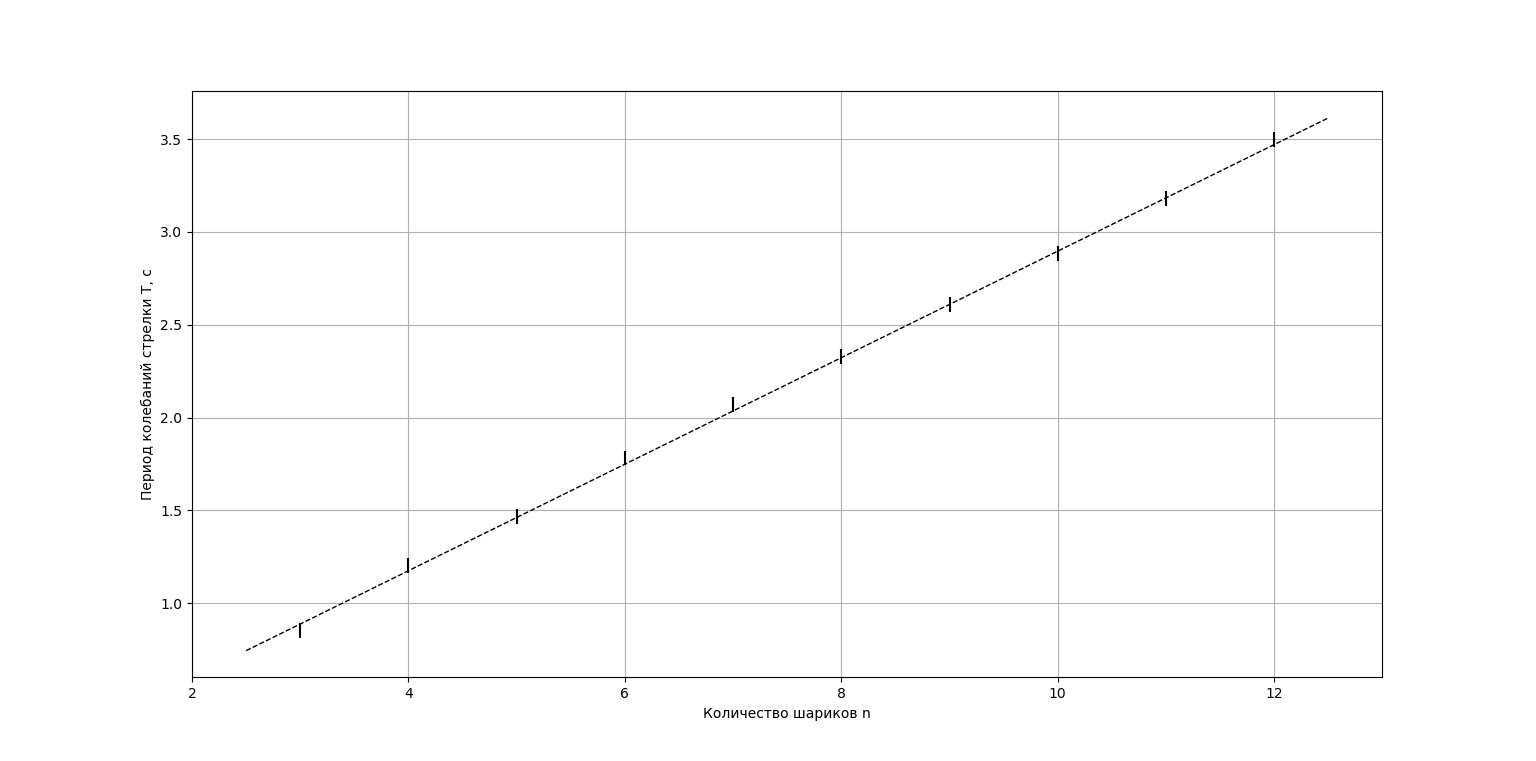
\includegraphics[scale = 0.33]{plot}
	\caption{Зависимость периода колебаний $T$ магнитной "стрелки" от числа шариков $n$, её составляющих. Прямая проведена по МНК} \label{plot}
\end{figure} 

\subsection*{III. Определение вертикальной составляющей магнитного поля Земли}

Изготовим из чётного числа $n$ шариков магнитную "стрелку" и подвесим её на штативе за середину с помощью нити. Далее, с помощью одного или нескольких кусков проволоки уравновесим "стрелку" в горизонтальном положении. С помощью весов определим массу уравновешивающего груза $m_{\text{гр}}$. Тогда, зная плечо силы тяжести $r_{\text{гр}}$, можно будет найти момент сил $M$, действующий на горизонтальную "стрелку" со стороны поля Земли. Для "стрелки" из $n$ шариков уравновешивающий груз будем подвешивать так, чтобы плечо силы тяжести равнялось $\left(\frac{n}{2}-1\right)d$.

Проведём вышеописанные измерения для чётных значений $n=$ 4, 6, 8, 10, 12. Результаты занесём в таблицу \Ref{ravn}. Зная погрешность весов и диаметра шарика, рассчитаем погрешности магнитного момента $M$. Также занесём их в таблицу.

\begin{table}[h]
	\centering
	\caption{Зависимость момента сил $M$, действующего на горизонтальную магнитную "стрелку", от количества шариков $n$, её составляющих} \label{ravn}
	\begin{tabular}{|c|c|c|c|c|c|c|c|c|c|c|}
		\hline
		$n$ & 4 & 6 & 8 & 10 & 12 \\ \hline
		$r_{\text{гр}}$, см & 0,59 & 1,19 & 1,78 & 2,38 & 2,97 \\ \hline
		$m_{\text{гр}}$, г & 0,218 & 0,160 & 0,147 & 0,134 & 0,129 \\ \hline
		$M$, $\text{дин}\cdot\text{см}$ & 127,0 & 186,4 & 256,9 & 312,2 & 375,7 \\ \hline
		$\sigma_M$, $\text{дин}\cdot\text{см}$ & 1,9 & 3,4 & 4,9 & 6,4 & 7,9 \\ \hline
	\end{tabular}
\end{table}

Построим график зависимости $M(n)$. Он приведён ниже на рисунке \Ref{plott}. Видим, что полученная зависимость линейна, из чего можно сделать вывод об аддитивности магнитных моментов для используемых в работе магнитов. Для нахождения углового коэффициента воспользуемся МНК, получим результат $A=\left(31,4\pm0,7\right)~\text{дин}\cdot\text{см}$.

\begin{figure}[h]
	\centering
	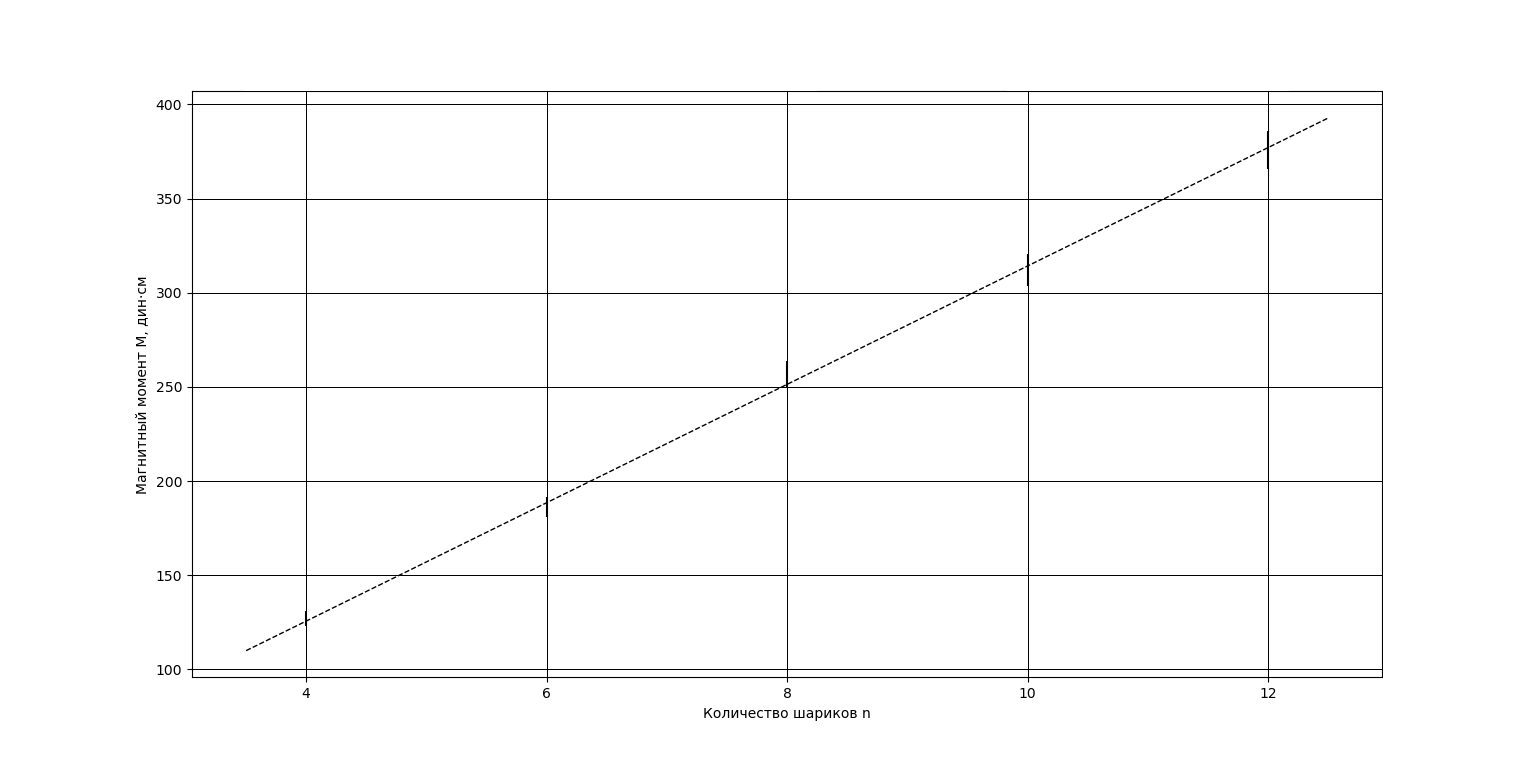
\includegraphics[scale = 0.33]{plott}
	\caption{Зависимость момента сил $M$, уравновешивающего магнитную "стрелку" , от числа шариков $n$, её составляющих. Прямая проведена по МНК} \label{plott}
\end{figure} 

Наконец, найдём вертикальную составляющую магнитного поля Земли по формуле\[B_v=\frac{A}{\mathfrak{m}}=\left(38,2\pm0,9\right)~\text{мкТл}.\]Отсюда уже несложно найти магнитное наклонение и полную величину индукции магнитного поля $\beta=\arctan{\frac{B_h}{B_v}}=\left(71,5\pm1,2\right)^{\circ}$ и $B=\sqrt{B_h^2+B_v^2}=\left(66,5\pm1,5\right)~\text{мкТл}$ в районе Долгопрудного соответственно. Табличное значения индукции магнитного поля Земли в Москве равно $B=65~\text{мкТл}$, а магнитного наклонения -- $\beta=72^{\circ}$, т.е. полученные в работе значения в пределах погрешности совпадают с табличными.

Оценим полный магнитный момент Земли:\[\mathfrak{m}_{\text{З}}=\frac{BR_{\text{З}}^3}{\sqrt{3\sin^2{\varphi}+1}}=\left(1,00\pm0,02\right)\cdot10^{26}~\text{ед. СГС},\]где $\varphi=56^{\circ}$ -- широта Москвы.

\section*{Вывод}

В данной работе были исследованы свойства постоянных неодимовых магнитов. В частности, были найдены свойства их материала -- например, остаточная индукция магнитного поля шариков равна $B_r=\left(1,02\pm0,02\right)~\text{Тл}$, что в пределах погрешности совпадает с табличным значением $B_{r0}=1,00~\text{Тл}$.

С помощью магнитных шариков были измерены горизонтальная и вертикальная составляющие поля Земли, были получены значения $B_h=\left(55,6\pm0,9\right)~\text{мкТл}$ и $B_v=\left(38,2\pm0,9\right)~\text{мкТл}$. Полная величина индукции магнитного поля Земли $B=\left(66,5\pm1,5\right)~\text{мкТл}$ и магнитное наклонение $beta=\left(71,5\pm1,2\right)^{\circ}$ совпадают в пределах погрешности с таличными значениями $B=65~\text{мкТл}$ и $\beta=72^{\circ}$ в Московском регионе.

Хорошее совпадение полученных в ходе работы результатов говорит о высокой точности используемых методов измерения.

\end{document}
